Pada Bab ini berisikan source code dari sistem yang di buat, source tersebut mencakup dari source code SQL atau database sistem kemudian dilanjutkan dengan source code Aplikasi yang terdiri dari source code dashboard, source code login, souce code CRUD tabel Alternatif, source code CRUD tabel user, source code CRUD tabel bobot, kemudian terakhir yaitu source code proses entropy, selain source code pada bab ini juga di tampilkan view atau user interface hasil dari source code tersebut.
\pagebreak

\section{Source Code Sql}

Pada bagian ini berisikan source code sql yang merupakan code dari sql untuk membuat tabel yang terdapat pada basis data sistem, kemudian dari source code tersebut terdapat source code untuk merelasikan tabel, sehingga jika source code sql tersebut di jalankan maka hasilnya berupa tiga tabel yang telah di relasikan. untuk lebih jelasnya berikut ini merupakan source code sql untuk sistem.

\lstinputlisting[caption=Source Code SQL Database System,label={sql}]{src/sql/db.sql}

\section{Source Code Aplikasi}
	kemudian jika telah membuat database dengan souce code \ref{sql} pada sub bab sebelumnya maka dilanjutkan dengan mengisikan source code Aplikasi pada file-file yang telah di buat sebelumnya source code aplikasi ini terdiri dari souce code yang terdapat pada controllers, model, view, dan library. maka dari itu berikut ini merupakan source code dari aplikasi.
\pagebreak

\subsection{Source Code Dashboard}

Langkah pertama yaitu membuat terlebih dahulu source code dashbord yang terdiri dari source code pada controller dan source code pada view, untuk lengkapnya berikut merupakan source code-nya.
\lstinputlisting[caption=File Controller Dashboard.php,label={das1}]{src/controllers/Dashboard.php}
pada source code \ref{das1} berikut merupakan sourcode pada bagian controller untuk dashboard.

\lstinputlisting[caption=File main.php,label={das2}]{src/views/layouts/main.php}
pada source code \ref{das2} berikut merupakan sourcode pada bagian view untuk dasar template, yang memunculkan side bar, nav bar dan bagian footer pada tampilan kemudian untuk content untuk keseluruhan aplikasi kecuali login di jalankan pada source code tersebut.

\lstinputlisting[caption=File View dashboard.php,label={das3}]{src/views/dashboard.php}
pada source code \ref{das3} tersebut merupakan souce code yang di gunakan untuk content atau isi dari dashboard atau halaman untuk setiap user, maka dari itu jika souce code telah selesai di buat untuk hasilnya seperti pada gambar \ref{ve5} untuk dashboard user kemudian untuk dashboard admin seperti pada gambar \ref{ve6}.

\begin{figure}[!htbp]
	\centerline{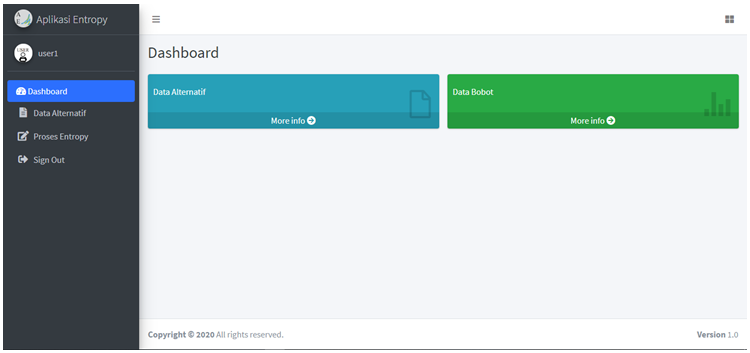
\includegraphics[width=0.90\textwidth]{figures/view/5.png}}
	\caption{view dashboard untuk user}
	\label{ve5}
\end{figure}

pada gambar \ref{ve5} merupakan tampilan dashboard untuk user, dimana pada dahboard tersebut menampilkan dua card didalamnya terdapat link untuk mengakses data alternatif dan data bobot.


\begin{figure}[!htbp]
	\centerline{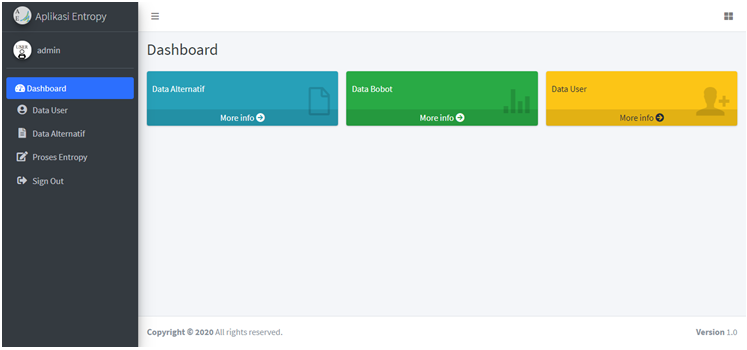
\includegraphics[width=0.90\textwidth]{figures/view/6.png}}
	\caption{view dashboard untuk admin}
	\label{ve6}
\end{figure}

pada gambar \ref{ve6} merupakan tampilan dashboard untuk admin , dimana pada dash board tersebut menampilkan tiga card didalamnya terdapat link untuk mengakses data alternatif, data bobot dan data user.
\pagebreak

\subsection{Source Code Login}
	Kemudian jika sudah membuat tampilan untuk dashboard dilanjutkan dengan membuat tampilan serta fungsi untuk login yang bertujuan agar dapat mengakses sistem serta dapat mgeakses tampilan dashboard yang bebeda dikarenakan userl lever yang berbeda.
\lstinputlisting[caption=File Controller Login.php,label={lo1}]{src/controllers/Login.php}
pada source code \ref{lo1} tersebut merupakan sourcode controller login yang di dalamnya terdiri dari kelas dan method-method login, kemudian untuk kunci session juga terdapat pada source code tersebut, yang di gunakan untuk membedakan tampilan untuk setiap user level-nya.
\lstinputlisting[caption=File Login\_model.php,label={lo2}]{src/models/Loginmodel.php}
pada source code \ref{lo2} tersebut merupakan model untuk login, yang di gunakan untuk membandingkan data dengan data yang terdapat pada tabel user yang di kirimkan oleh form login dan telah di proses di controller, jika data yang di bandingkan pada model maka akan di kirimkan ke controller kemudian user tidak akan bisa login atau masuk ke sistem.
\lstinputlisting[caption=File View login.php,label={lo3}]{src/views/login.php}
pada source code \ref{lo3} tersebut merupakan source code untuk form login atau tampilan form login, untuk hasilnya seperti pada gambar \ref{ve7}, dimana pada gambar tersebut terdiri dari dua form input yaitu username dan passwor untuk user.
\pagebreak
\lstinputlisting[caption=File library enkripsi.php,label={lo4}]{src/libraries/enkripsi.php}
pada source code \ref{lo4} tersebut merupakan class atau soucode pada folder library yang di gunakan untuk mengenkripsi password menjadi kode-kode kemudian di simpan pada database kemudian fungsi tersebut juga di gunakan untuk mengurai code password sehingga bisa di munculkan seperti code asalnya.

\begin{figure}[!htbp]
	\centerline{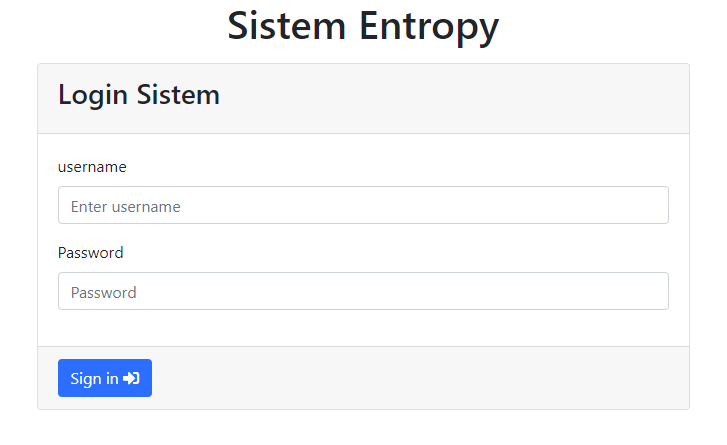
\includegraphics[width=0.90\textwidth]{figures/view/7.png}}
	\caption{Form Login Sistem}
	\label{ve7}
\end{figure}

\textbf{Catatan :}\par
\textit{Untuk Source code enkripsi hanya bisa di gunakan pada PHP 5 untuk versi PHP 7 tidak bisa menggunakan source code tersebut}
\pagebreak

\subsection{Source Code CRUD Tabel Alternatif}
	kemudian setelah source codelogon di buat maka di lanjutkan dengan membuat source code untuk mengelola data alternatif, yang mana data ini di gunakan untuk menentukan bobot dari setiap kriteria, untuk hak akses dalam mengelola data ini terbagi dua. untuk admin dapat mengelola keseluruhan data yang di miliki oleh user lain, sedangkan untuk user pengguna biasa hanya bisa mengelola data yang di miliki oleh user tersebut. agar lebih jelas berikut merupakan source code dari CRUD ( create, read, update, dan delete).
\lstinputlisting[caption=File Controller Tbl\_alternatif.php,label={asdw}]{src/controllers/Tbl_alternatif.php}
	pada source code \ref{asdw} tersebut merupakan sourcode controller dari pengelolaan data alternatif dimana di dalamnya terdiri dari fungsi-fungsi yang di gunakan untuk memunculkan data, menambahkan data, mengedit data kemudian menghapus data.
\lstinputlisting[caption=FileTbl\_alternatif\_model.php,label={asdw1}]{src/models/Tbl_alternatif_model.php}
	Pada source code \ref{asdw1} tersebut merupakan sourcode dari model yang di gunakan untuk mengelola data alternatif, yang terdiri dari fungsi fungsi yang berhubungan langsung dengan basis data dan controller dalam mengelola data dari tabel alternatif.
\lstinputlisting[caption=File View tbl\_alternatif index.php,label={asdw3}]{src/views/tbl_alternatif/index.php}
	Source code \ref{asdw3} tersebut di gunakan untuk desain halaman utama untuk data alternatif dimana data tersebut di tampilkan dalam bentuk tabel, kemudian untuk tampilannya sendiri terdiri dari dua tampilan bedasarkan user level. untuk userllevel admin maka data alternatif dari semua user akan di munculkan seperti pada gambar \ref{ve8} kemudian untuk user pengguna atau selai admin hanya akan menampilkan data yang terdaftar sebagai user itu sendiri seperti pada gambar \ref{ve9} berikut.
\begin{figure}[!htbp]
	\centerline{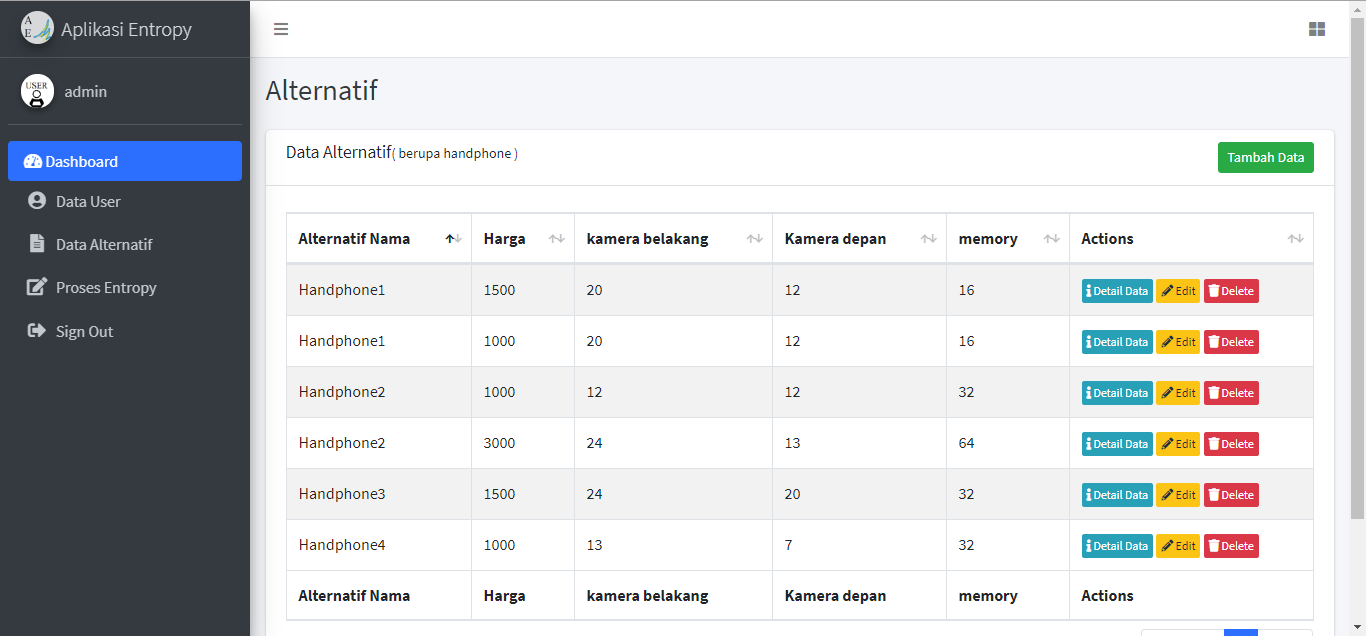
\includegraphics[width=0.90\textwidth]{figures/alt/idx1.png}}
	\caption{tampilan utama data index pada admin}
	\label{ve8}
\end{figure}

\begin{figure}[!htbp]
	\centerline{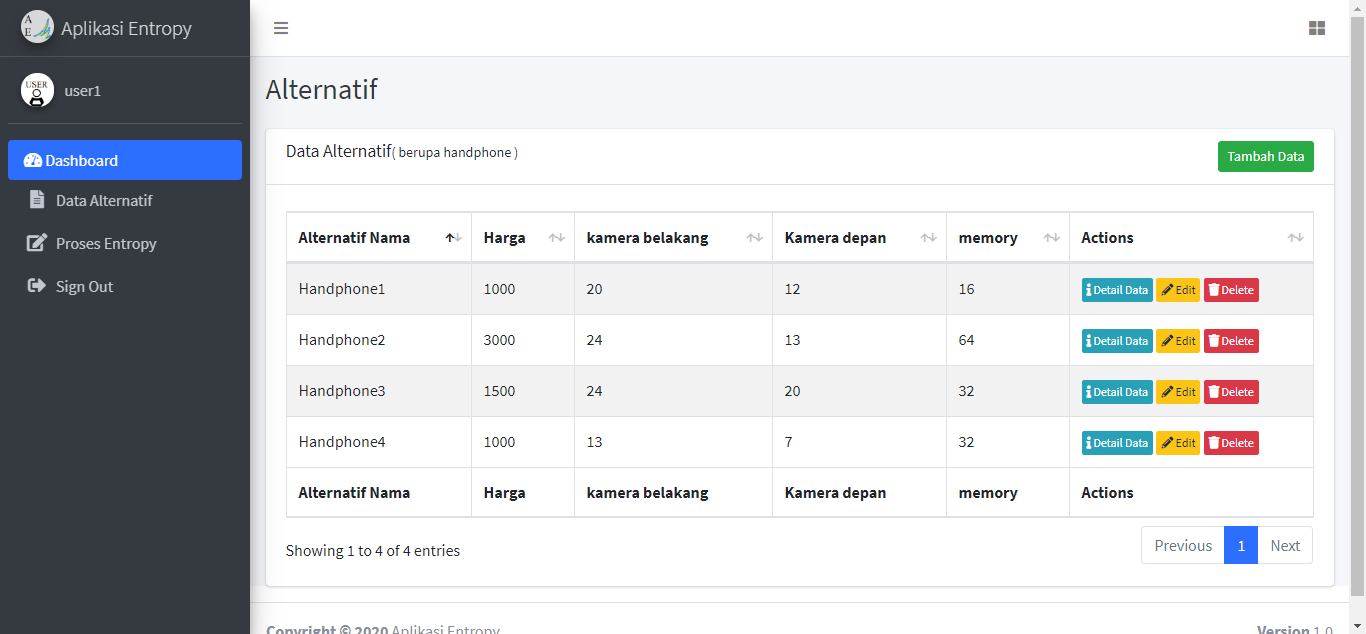
\includegraphics[width=0.90\textwidth]{figures/alt/idx2.png}}
	\caption{tampilan utama data index pada user}
	\label{ve9}
\end{figure}
\pagebreak
\lstinputlisting[caption=File View tbl\_alternatif add.php,label={asdw4}]{src/views/tbl_alternatif/add.php}
lalu setelah tampilan utama untuk data alternatif maka ada tampilan dari form untuk menambah data alternatif, dari tampilan untuk menambahkan data alternatif dari form input dan seterusnya untuk userlevel yang berbeda tidak ada perbedaan di bagian input data, untuk pengelolaan data alternatif bedanya hanya pada saat data di tampilkan dalam kondisi sudah melakukan login pada sistem.\par
\begin{figure}[!htbp]
	\centerline{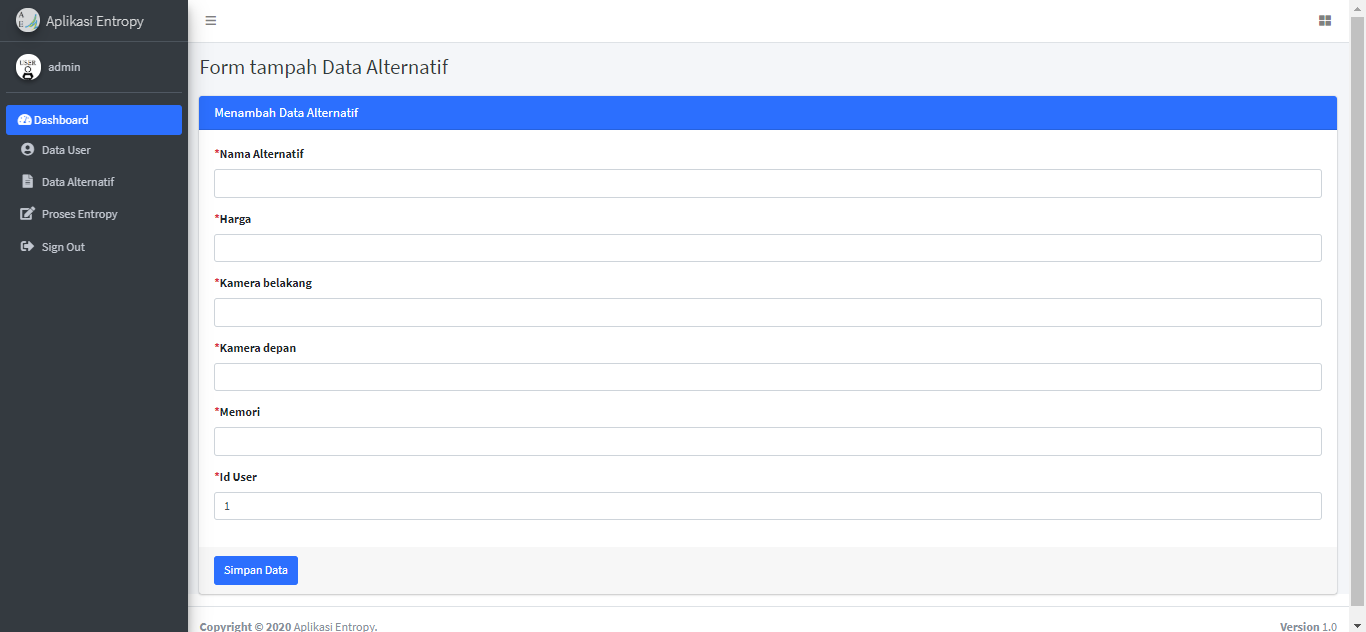
\includegraphics[width=0.90\textwidth]{figures/alt/add.png}}
	\caption{tampilan form tambah data}
	\label{ve10}
\end{figure}
pada gambar \ref{ve10} tersebut merupakan tmpilan dari form tambah data yang source codenya yaitu souce code \ref{asdw4} tersebut.\par

kemudian jika telah membuat source code untuk menambah data di lanjutkan dengan membuat source code \ref{asdw5} yang di gunakan untuk membuat form edit data pada dasarnya form edit hampir sama dengan form tambah data hanya saja berbeda pada fungsi controller yang di tuju, kemudian pada form biasanya telah terisi data.
\lstinputlisting[caption=File View tbl\_alternatif edit.php,label={asdw5}]{src/views/tbl_alternatif/edit.php}

\begin{figure}[!htbp]
	\centerline{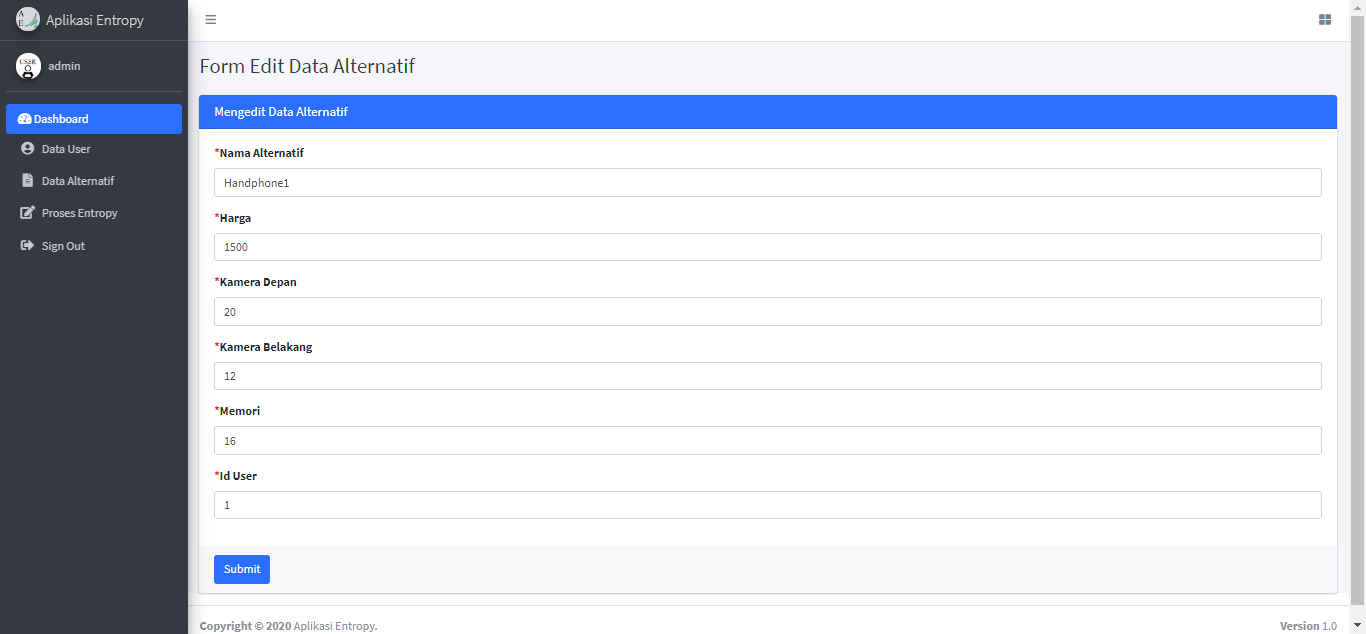
\includegraphics[width=0.90\textwidth]{figures/alt/edit.png}}
	\caption{tampilan form edit data}
	\label{ve11}
\end{figure}

untuk hasi ldari form edit data maka seperti pada gambar \ref{ve11} tersebut, yang sekilas mirip dengan form tambah data pada gambar \ref{ve10}.\\


dikarenakan data yang di tampilkan pada tabel bukan keseluruhan data, maka dibutuhkan fitur detail data yang di gunakan untuk melihat detai dari setiap data alternatif, kemudian untuk source code dari detai data alternatif tersebut seperti pada source code \ref{asdw6} berikut ini.
\lstinputlisting[caption=File View tbl\_alternatif detail.php,label={asdw6}]{src/views/tbl_alternatif/detail.php}

jika source code detail data alternatif telah di implementasikan makahasinya seperti pada gambar \ref{ve12} berikut ini, yang berupa tabel yang berisikan detai dari satu data alternatif yang di pilih.
\begin{figure}[!htbp]
	\centerline{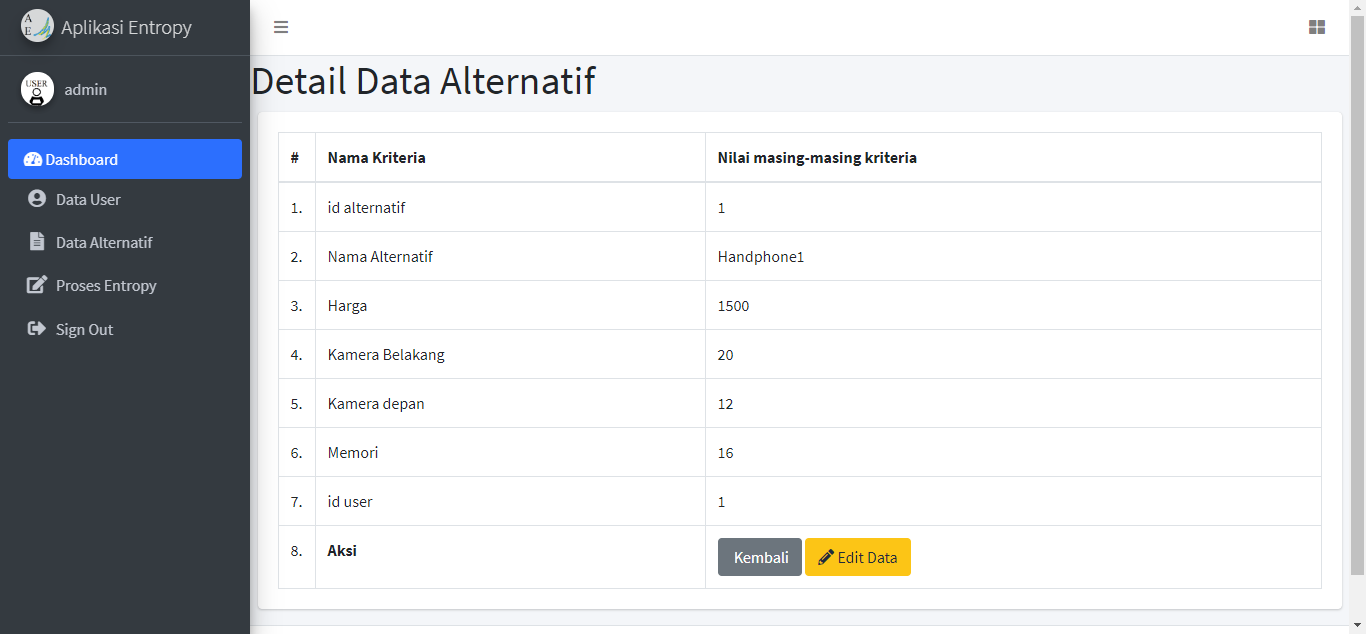
\includegraphics[width=0.80\textwidth]{figures/alt/detail.png}}
	\caption{tampilan detail data}
	\label{ve12}
\end{figure}
\pagebreak

\subsection{Source Code CRUD Tabel User}
	setelah data alternatif maka selanjutnya source code crud dari tabel user, dimana untuk mengelola datauser hanya bisa di lakukan oleh user admin saja untuk user lain tidak ada akses untuk melakukan pengelolaan data tersebut, maka dari itu berikut merupakan source code yang di gunkan dalam mengelola data user.
\lstinputlisting[caption=File Controller Tbl\_user.php,label={U1}]{src/controllers/Tbl_user.php}
	pada source code \ref{U1} merupakan controller yang di gunakan untuk mengelola data user, untuk logikanya sama saja seperti pada controller untuk mengelola data alternatif, pada controller ini juga terdapat beberapa fungsi yang di gunakan untuk aktifitas CRUD data user.
\lstinputlisting[caption=FileTbl\_user\_model.php,label={U2}]{src/models/Tbl_user_model.php}
	Pada source code \ref{U2} tersebut merupakan model yang di gunakan oleh controller tbl\_user, pada model tersebut terdapat beberapa fungsi yang di gunakan untuk memunculkan data, memunculkan data berdasarkan id, mengedit data, menyimpan data hingga untuk menghapus data user.
\lstinputlisting[caption=File View tbl\_user index.php,label={U3}]{src/views/tbl_user/index.php}
	pada source code \ref{U3} tersebut merupakan source code yang di gunakan untuk menampilkan data user, data tersebut di tampilkan dalam bentuk tabel yang di sertai dengan tombol-tombol yang di gunakan untuk berpindah ke halaman edit data, detail data, tambah data, hingga untuk menghapus data user. kemudian untuk hasil dari source code tersebut maka tampilannya seperti pada gambar \ref{ve13} berikut ini.\par
\pagebreak
\begin{figure}[!htbp]
	\centerline{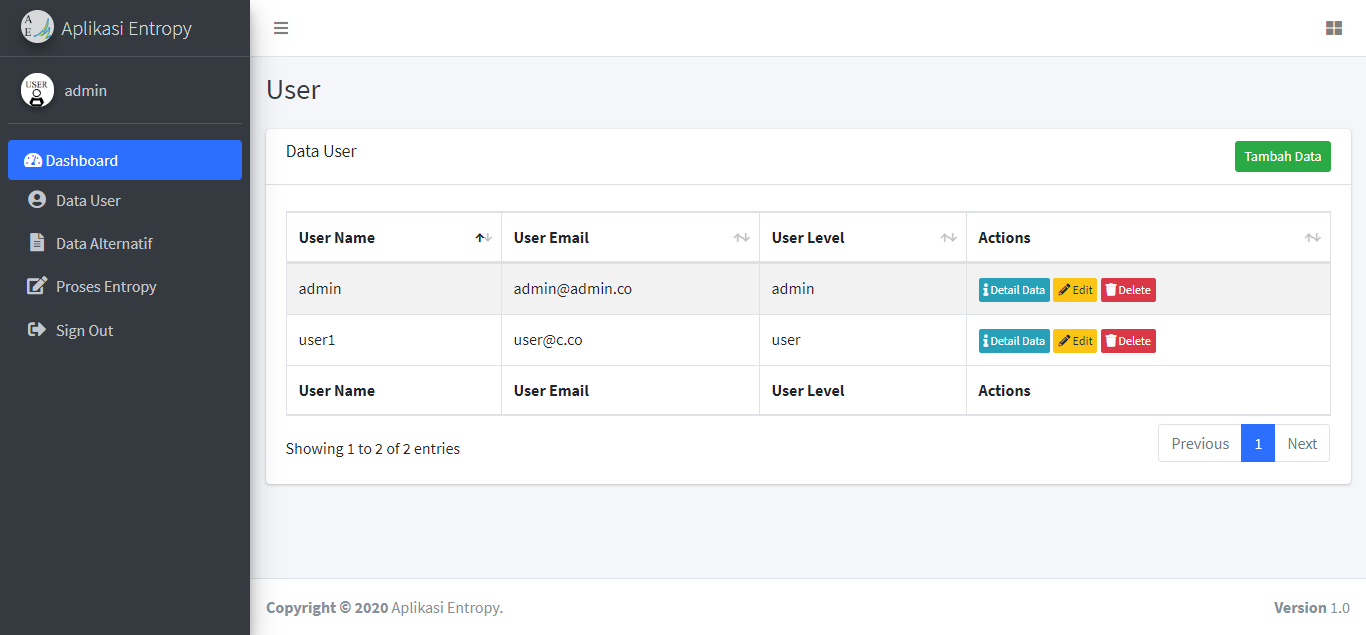
\includegraphics[width=0.90\textwidth]{figures/us/idx.png}}
	\caption{tampilan utama data index pada admin}
	\label{ve13}
\end{figure}
Pada gambar \ref{ve13} tersebut merupakan halaman utama untuk data user yang di gunakan untuk menampilkan data user serta fitur untuk mengelola data user.


\lstinputlisting[caption=File View tbl\_user add.php,label={U4}]{src/views/tbl_user/add.php}
	setelah tampilan data user dilanjutkan dengan membuat form tambah data user, untuk source codenya seperti pada source code \ref{U4} berikut yang merupakan source code untuk form tambah data user, yang hasil dari source code tersebut seperti pada gambar \ref{ve14} berikut ini.
\pagebreak
\begin{figure}[!htbp]
	\centerline{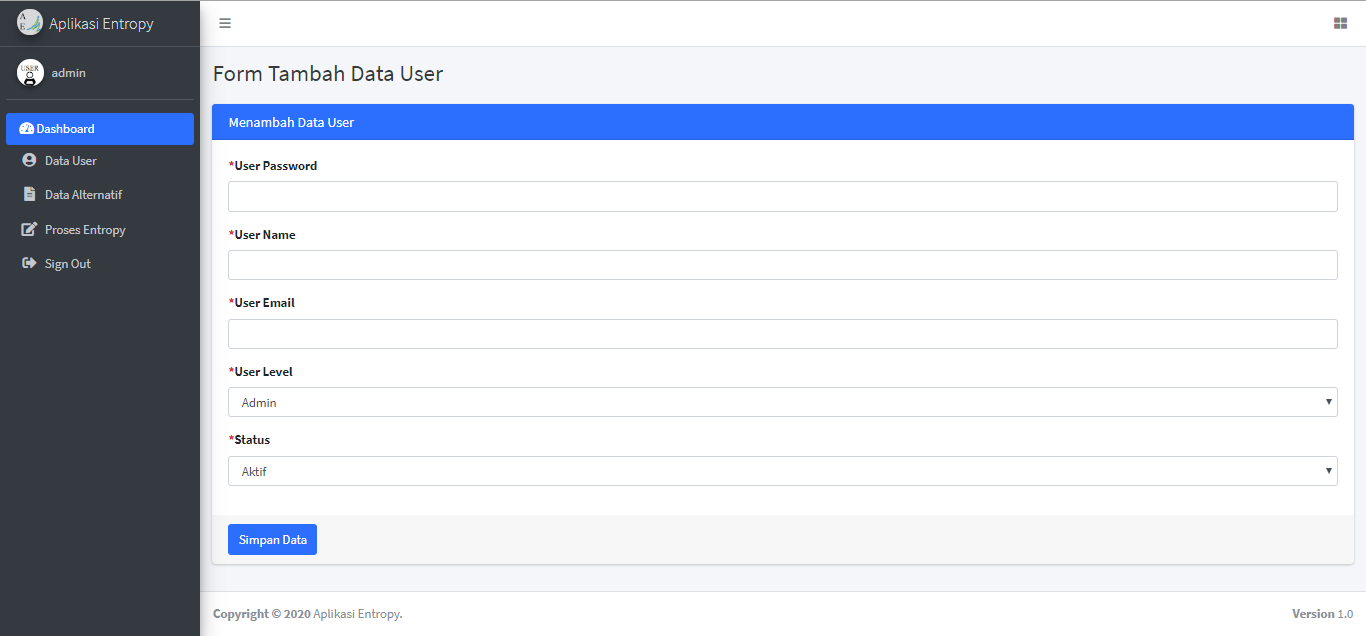
\includegraphics[width=0.90\textwidth]{figures/us/add.png}}
	\caption{tampilan form tambah data}
	\label{ve14}
\end{figure}

pada gambar \ref{ve14} tersebut merupakan form tambah data untuk menambah data user, untuk form ini hanya bisa di akses oleh user admin saja.

\lstinputlisting[caption=File View tbl\_user edit.php,label={U5}]{src/views/tbl_user/edit.php}
	jika form tambah data user telah di buat di lanjutkan dengan membuat form untuk mengedit data, pada source code \ref{U5} tersebut merupakan code yang digunakan untuk membuat form edit data, kalau pada dasarnya form edit data dan tambah data hampirsama hnyasaja beda fungsi untuk mengirim data dan pada form edit data biasanya telah terdapat data yang siap untuk di ubah pada form yang telah di pilih. lalu untuk hasil dari souce code tersebut terdapat pada gambar \ref{ve15} berikut.\par
\begin{figure}[!htbp]
	\centerline{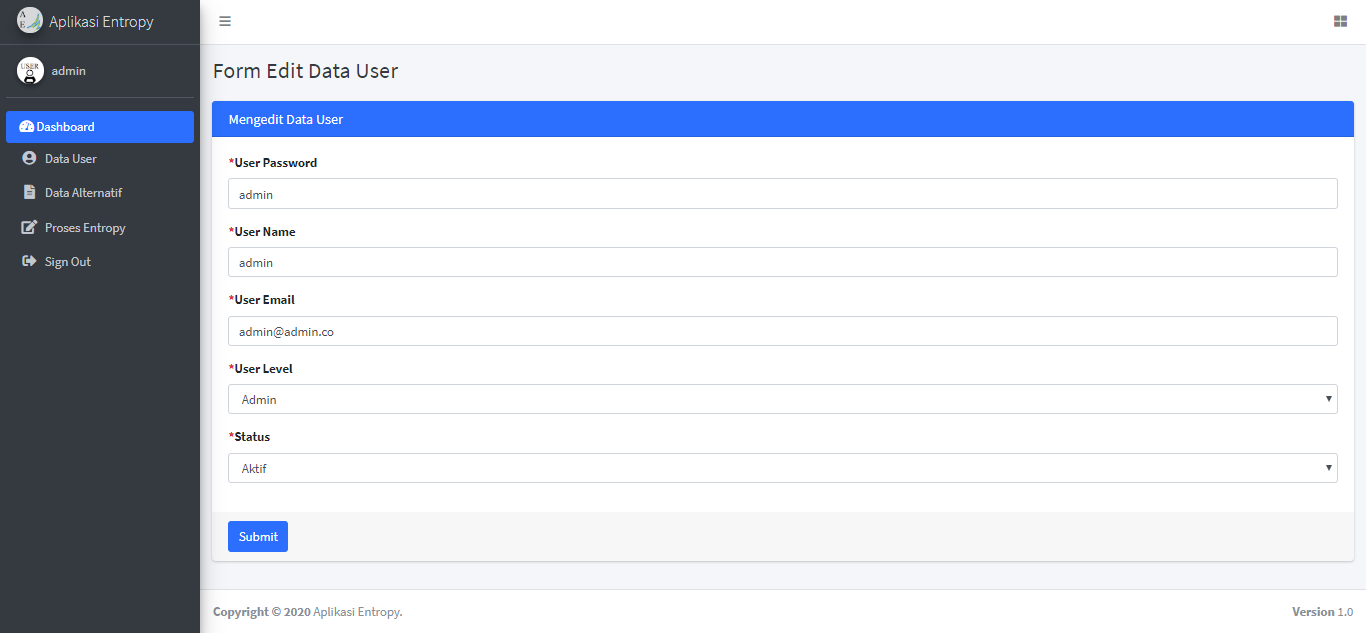
\includegraphics[width=0.90\textwidth]{figures/us/edit.png}}
	\caption{tampilan form edit data}
	\label{ve15}
\end{figure}
 pada gambar \ref{ve15} berikut merupakan form edit hasil dari source code \ref{U5}.
\lstinputlisting[caption=File View tbl\_user detail.php,label={U6}]{src/views/tbl_user/detail.php}
kemudian dikarenakan pada tabel user data user tidak di tampilkan semua maka ada fitur untuk detail data maka dari itu pada source code \ref{U6} tersebut merupakan source code yang di gunakan untuk membuat tampilan dari detail data user, untuk hasilnya seperti pada gambar \ref{ve16} berikut.\par
\begin{figure}[!htbp]
	\centerline{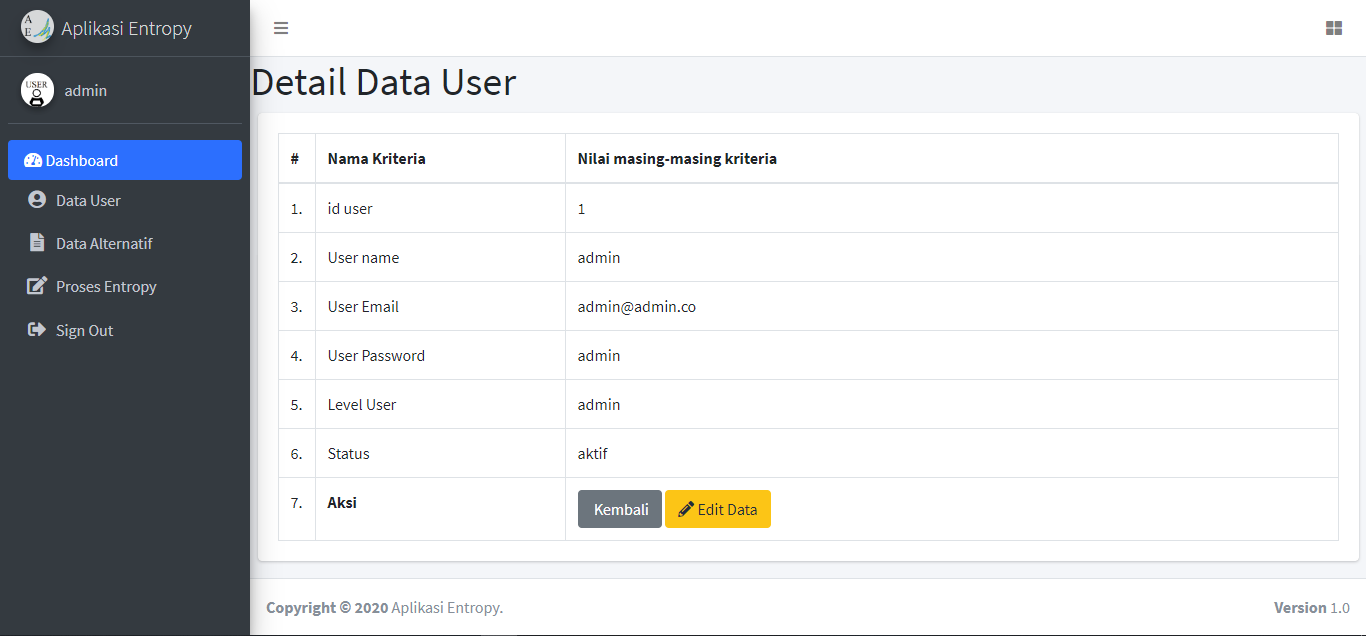
\includegraphics[width=0.90\textwidth]{figures/us/detail.png}}
	\caption{tampilan detail data}
	\label{ve16}
\end{figure}
pada gambar \ref{ve16} berikut merupakan tampilan dari detail data user yang di tampilkan dalam bentuk tabel data.

\subsection{Source Code CRUD Tabel Bobot}
	setelah membuat source code untuk alternatif di lanjutkan dengan membuat source code untuk bobot taua source code CRUD tabel bobot, yang sebenarnya untuk data bobot yang di simpan pada fitur ini berasal dari data hasil perhitungan entropy, fitur ini di buat karena untuk antisipasi pembulatan nilai bobot atau untuk menyesuaikan nilai bobot hasilperhitungan entropy. maka dari itu berikut merupakan source code daru tabel bobot.
\lstinputlisting[caption=File Controller Tbl\_bobot.php,label={B1}]{src/controllers/Tbl_bobot.php}
yang pertama yaitu source code \ref{B1}  pada controller dimana source code tersebut hampir sama fungsinya seperti soucode controller untuk tabel alternatif maupun tabel user.
\lstinputlisting[caption=FileTbl\_bobot\_model.php,label={B2}]{src/models/Tbl_bobot_model.php}
kemudian model dari tabel bobot yang merupakan yang fungsinya juga hampirsama seperti model-model pada tabel sebelumnya yang di gunakan untuk menampilkan data mengedit data dan menghapus data.
\lstinputlisting[caption=File View tbl\_bobot index.php,label={B3}]{src/views/tbl_bobot/index.php}
lalu pada source code \ref{B3} merupakan source code yang di gunakan untuk menampilkan data bobot yang telah di simpan di basis data kemudian di tampilkan beserta fitur-fitur lainnya seperti edit delete dan fitur menambah data.
\begin{figure}[!htbp]
	\centerline{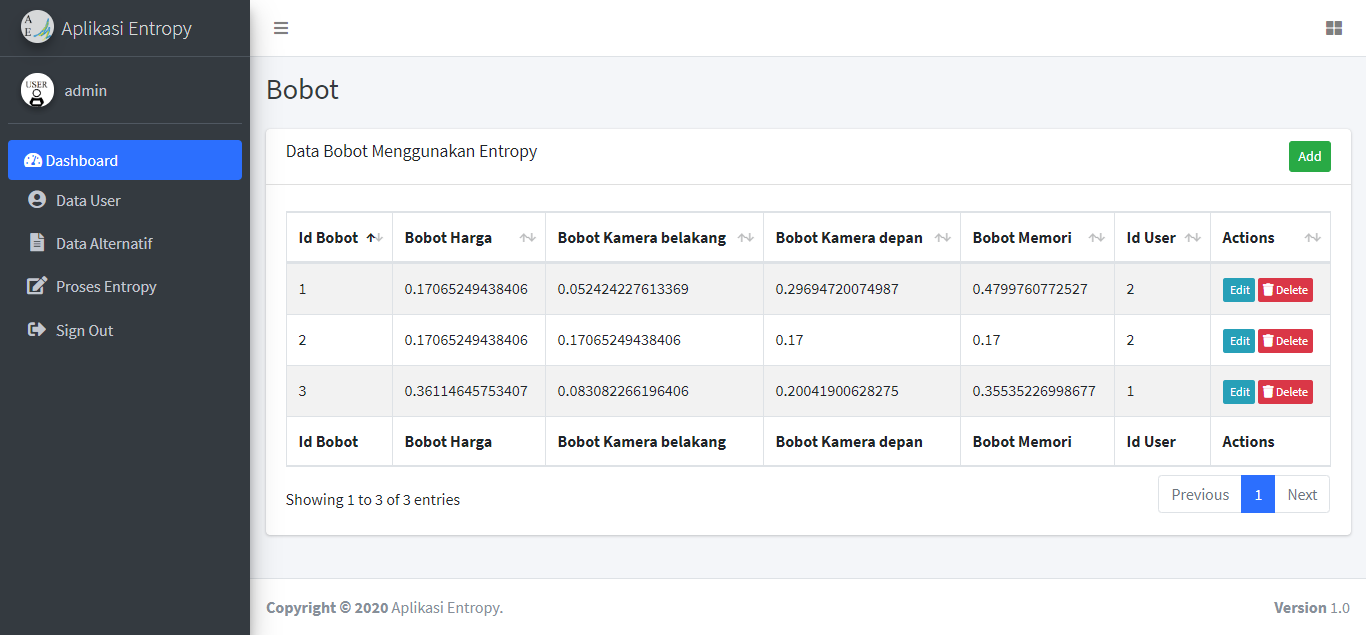
\includegraphics[width=0.90\textwidth]{figures/bo/idx.png}}
	\caption{tampilan form edit data}
	\label{ve17}
\end{figure}
pada gambar \ref{ve17} tersebut merupakan gambar dari tampilan utama untuk memunculkan data bobot yang di sertai dengan fitur edit, delete dan tambah data.


\lstinputlisting[caption=File View tbl\_bobot add.php,label={B4}]{src/views/tbl_bobot/add.php}

pada source code \ref{B4} tersebut merupakan source code untuk form tambah data bobot, form ini hampir sama seperti form pada umumnya yang di gunakan pada tabel alternatif dan tabel user, lalu untuk hasilnya seperti pada gambar \ref{ve18} berikut.
\begin{figure}[!htbp]
	\centerline{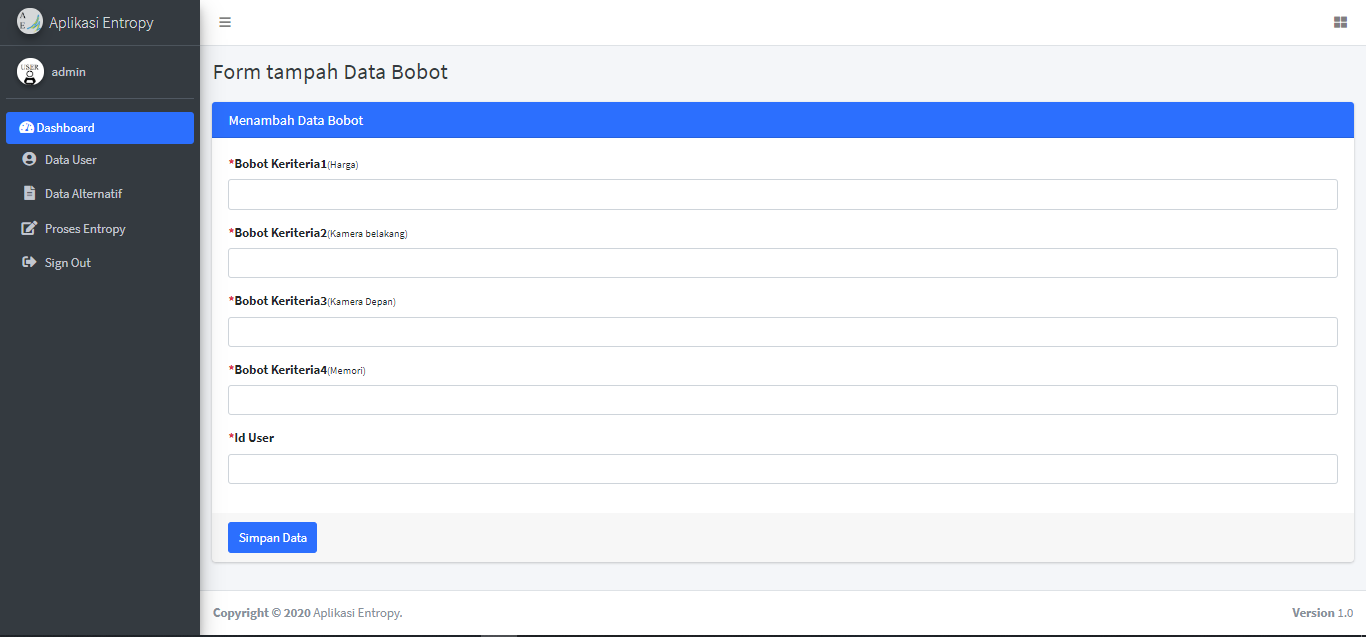
\includegraphics[width=0.90\textwidth]{figures/bo/add.png}}
	\caption{tampilan form tambah data}
	\label{ve18}
\end{figure}

\lstinputlisting[caption=File View tbl\_bobot edit.php,label={B5}]{src/views/tbl_bobot/edit.php}

pada source code \ref{B5} tersebut merupakan form edit data bobot ini juga hampir sama dengan form bobot yang di gunakan pada form bobot untuk tabel alternatif dan tabel user, hanya saja beda konten yang di tampilkannya. kemudian untuk hasilnya seperti pada gambar \ref{ve19} berikut ini.
\begin{figure}[!htbp]
	\centerline{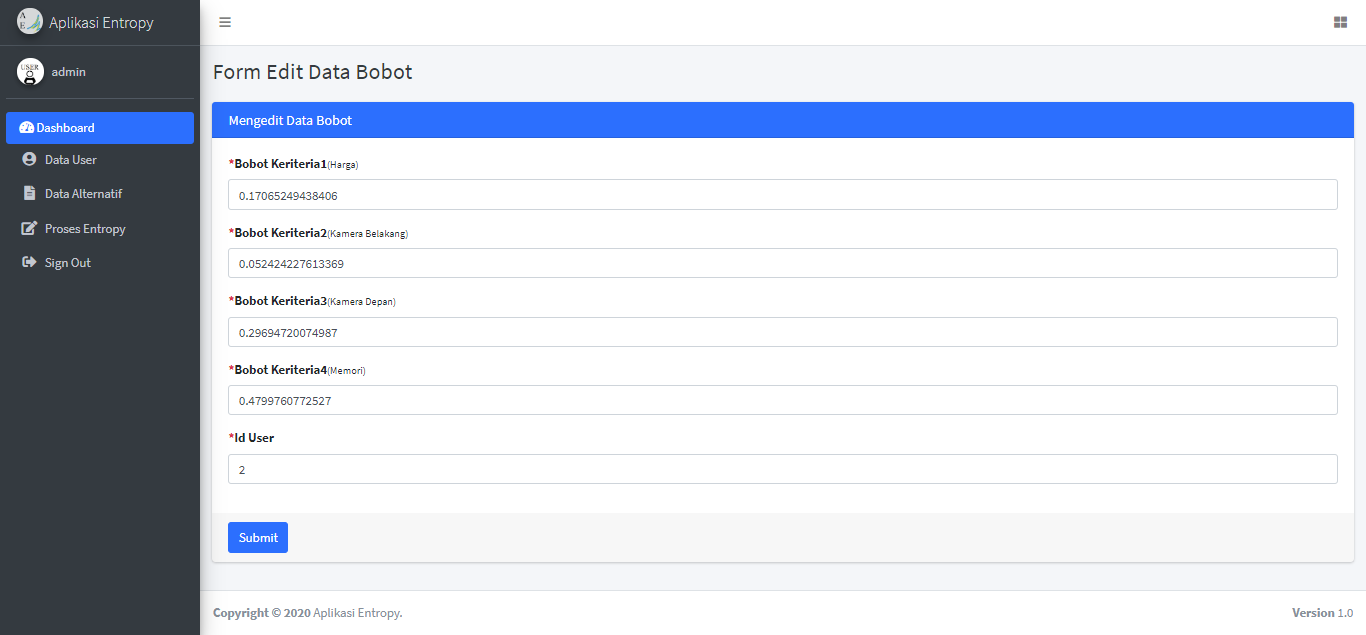
\includegraphics[width=0.90\textwidth]{figures/bo/edit.png}}
	\caption{tampilan form edit data}
	\label{ve19}
\end{figure}


\subsection{Source Code Proses Entropy}
	Setelah membuat source code untuk menampilkan serta mengelola data maka di lanjutkan pada pembuatan source code entropy yang merupakan metode untuk memberikan bobot pada kriteria dalam mengambil keputusan, agar lebih jelas berikut ini merupakan source code dalam metode entropy yang di praktekan melalui pemerograman php.
\lstinputlisting[caption=File Controller Proses\_entropy.php,label={q1}]{src/controllers/Proses_entropy.php}
pada source code \ref{q1} tersebut merupakan code dari controller dari entropy dimana logika entropy tersebut di simpan pada fungsi yang terdapat pada fungsi ini, lebih jelasnya pada fungsi proses dan proses user merupakan logika dari metode entropy ini yang merupakan rumusan entropy yang telah di bahas pada bab 3 dan bab 2 sebagai contoh dan materi kemudian di jabarkan menjadi source code maka hasilnya seperti pada source code tersebut.

\lstinputlisting[caption=File Entropy\_model.php,label={q2}]{src/models/Entropy_model.php}
pada source code \ref{q2} merupakan code dari model entropy, pada model tersebut data di tentukan diambil berdasarkan id kemudaian diambil nilai total untuk setiap data kriteria dimana data tersebut di seleksi berdasarkan id user, dimana jika parameter id user sudah terpenuhi dan pengambilan data telah dilakukan pada controller maka data-data kriteria tersebut di kirimkan lagi ke controller kemudian dilakukan proses perhitungan maka akhirnya akan mendapatkan nilai bobot untuk masing-masing kriteria dari perhitungan tersebut.

\lstinputlisting[caption=File View Entropy  index.php,label={q3}]{src/views/entropy/index.php}
pada source code \ref{q3} tersebut merupakan source code index entropy yang merupakan form input untuk id user, dimana hal tersebut merupakan syarat untuk memulai proses entropy tapi hal ini dilakukan hanya pada user admin saja karena data alternatif pada admin memunculkan semua data alternatif dari semua user sehingga untuk menghitung entropy untuk setiap user dilakukan seleksi data berdasarkan id user terlebi dahulu.
\begin{figure}[!htbp]
	\centerline{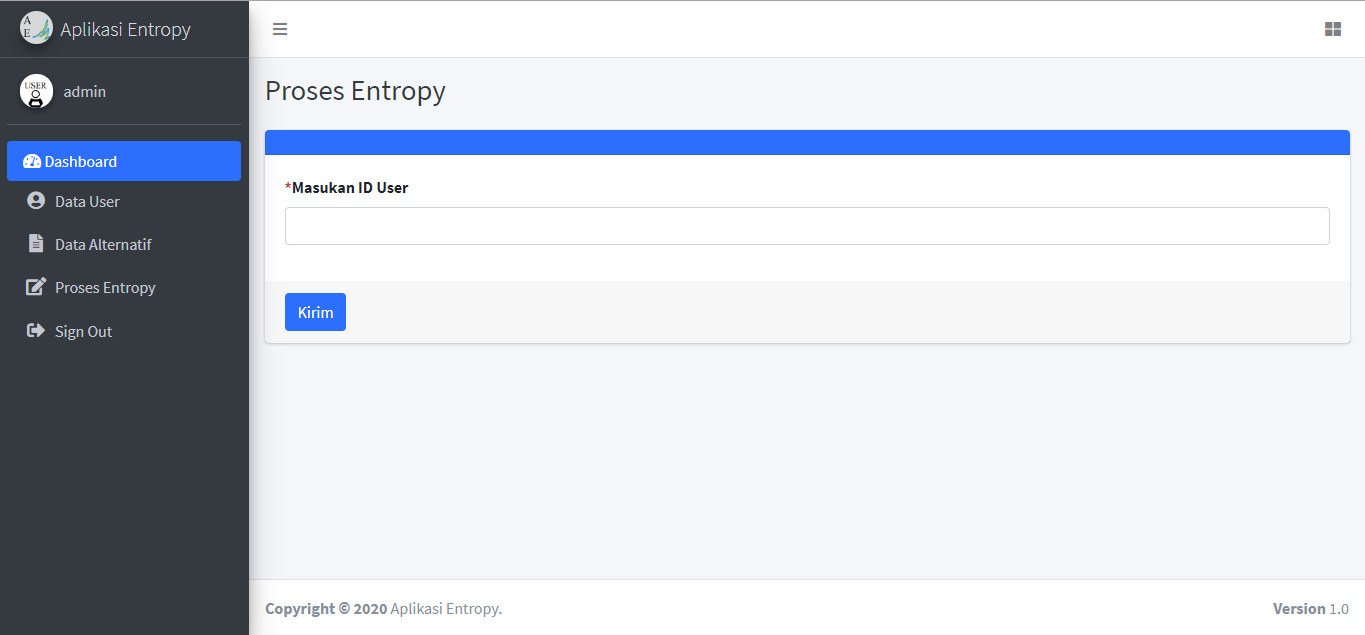
\includegraphics[width=0.90\textwidth]{figures/en/1.png}}
	\caption{Form input id user}
	\label{py1}
\end{figure}

pada gambar \ref{py1} merupakan proses entropy yang di lakukan pada user admin lalu perbedaan dengan user biasa yaitu userbiasa tidak perlu melakukan penyortiran data maka proses entropy akan berjalan dikarenakan menggunakan parameter id user yang melakukan login.
\pagebreak

\lstinputlisting[caption=File View Entropy  hasil.php,label={q4}]{src/views/entropy/hasil.php}

pada source code \ref{q4} merupakan code yang di gunakan untuk memunculkan view hasil dari perhitungan entropy, pada hasil tersebut data di simpan pada form di dalam tabel kemudian data tersebut bisa disimpan pada tabel bobot sehingga dapat bobot tersebut dapat dikelola dengan sistem crud bobot yang telah di buat sebelumnya.
\begin{figure}[!htbp]
	\centerline{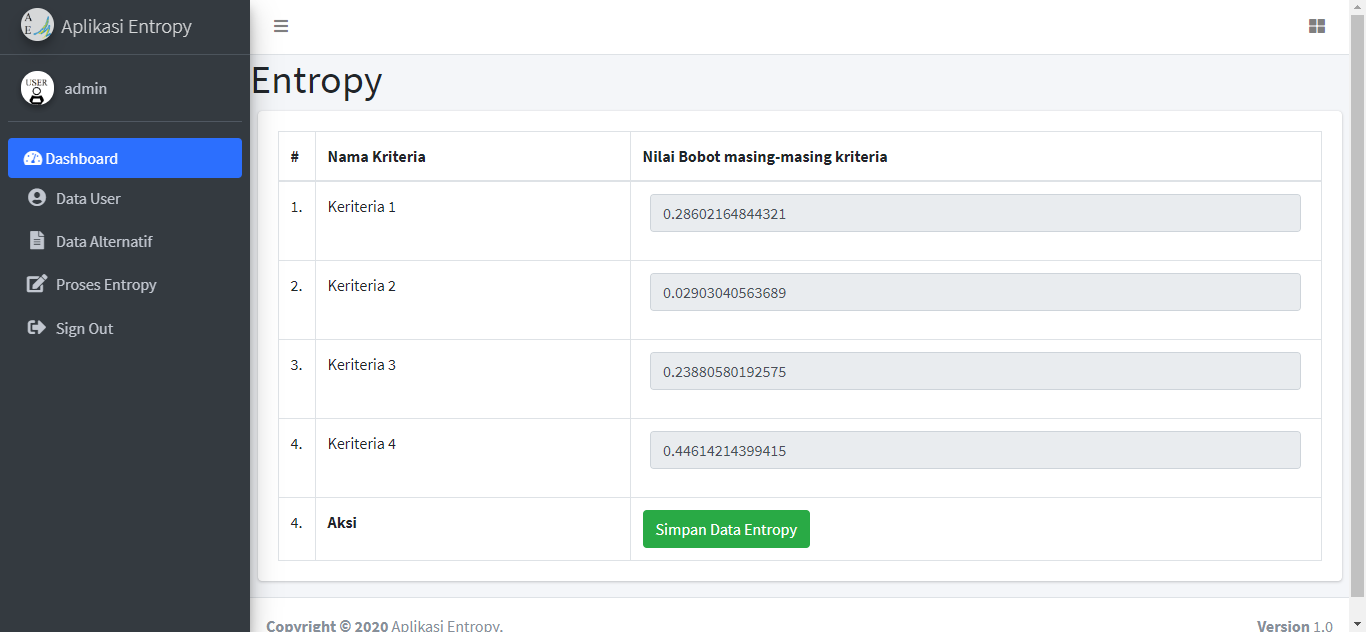
\includegraphics[width=0.90\textwidth]{figures/en/2.png}}
	\caption{Data entropy hasil perhitungan}
	\label{py2}
\end{figure}


